\documentclass[25pt, a0paper, landscape]{tikzposter}
\tikzposterlatexaffectionproofoff
\usepackage[utf8]{inputenc}
\usepackage{authblk}
\makeatletter
\renewcommand\maketitle{\AB@maketitle} % revert \maketitle to its old definition
\renewcommand\AB@affilsepx{\quad\protect\Affilfont} % put affiliations into one line
\makeatother
\renewcommand\Affilfont{\Large} % set font for affiliations
\usepackage{amsmath, amsfonts, amssymb}
\usepackage{tikz}
\usepackage{pgfplots}
% align columns of tikzposter; needs two compilations
\usepackage[colalign]{column_aligned}
\usepackage{graphicx}
\usepackage{caption}
\usepackage{subfig}
\usepackage{caption}
\usepackage{float}
\usepackage{amsmath}
\usepackage[most]{tcolorbox}
\usepackage{cite}


\tcbset{colback=yellow!10!white, colframe=red!50!black,
        highlight math style= {enhanced, %<-- needed for the ’remember’ options
            colframe=red,colback=red!10!white,boxsep=0pt}
        }

% tikzposter meta settings
\usetheme{Default}
\usetitlestyle{Default}
\useblockstyle{Default}

%%%%%%%%%%% redefine title matter to include one logo on each side of the title; adjust with \LogoSep
\makeatletter
\newcommand\insertlogoi[2][]{\def\@insertlogoi{\includegraphics[#1]{#2}}}
\newcommand\insertlogoii[2][]{\def\@insertlogoii{\includegraphics[#1]{#2}}}
\newlength\LogoSep
\setlength\LogoSep{-70pt}

\renewcommand\maketitle[1][]{  % #1 keys
    \normalsize
    \setkeys{title}{#1}
    % Title dummy to get title height
    \node[inner sep=\TP@titleinnersep, line width=\TP@titlelinewidth, anchor=north, minimum width=\TP@visibletextwidth-2\TP@titleinnersep]
    (TP@title) at ($(0, 0.5\textheight-\TP@titletotopverticalspace)$) {\parbox{\TP@titlewidth-2\TP@titleinnersep}{\TP@maketitle}};
    \draw let \p1 = ($(TP@title.north)-(TP@title.south)$) in node {
        \setlength{\TP@titleheight}{\y1}
        \setlength{\titleheight}{\y1}
        \global\TP@titleheight=\TP@titleheight
        \global\titleheight=\titleheight
    };

    % Compute title position
    \setlength{\titleposleft}{-0.5\titlewidth}
    \setlength{\titleposright}{\titleposleft+\titlewidth}
    \setlength{\titlepostop}{0.5\textheight-\TP@titletotopverticalspace}
    \setlength{\titleposbottom}{\titlepostop-\titleheight}

    % Title style (background)
    \TP@titlestyle

    % Title node
    \node[inner sep=\TP@titleinnersep, line width=\TP@titlelinewidth, anchor=north, minimum width=\TP@visibletextwidth-2\TP@titleinnersep]
    at (0,0.5\textheight-\TP@titletotopverticalspace)
    (title)
    {\parbox{\TP@titlewidth-2\TP@titleinnersep}{\TP@maketitle}};

    \node[inner sep=0pt,anchor=west]
    at ([xshift=-\LogoSep]title.west)
    {\@insertlogoi};

    \node[inner sep=0pt,anchor=east]
    at ([xshift=\LogoSep]title.east)
    {\@insertlogoii};

    % Settings for blocks
    \normalsize
    \setlength{\TP@blocktop}{\titleposbottom-\TP@titletoblockverticalspace}
}
\makeatother
%%%%%%%%%%%%%%%%%%%%%%%%%%%%%%%%%%%%%


% color handling
\definecolor{TumBlue}{cmyk}{1,0.43,0,0}
\colorlet{blocktitlebgcolor}{TumBlue}
\colorlet{backgroundcolor}{white}

% title matter
\title{Semester Project for DL4CV WS17/18}

\author[1]{Haoran Chen}
\author[1]{Lixin Xue}
\author[1]{Kai Wu}
\author[1]{Pengyuan Wang}
\author[1]{Yingqiang Gao}

\affil[1]{Technical University of Munich}

\insertlogoi[width=15cm]{tum_logo}
\insertlogoii[width=15cm]{tum_logo}


% main document
\begin{document}

\maketitle

\begin{columns}
\column{0.35}
\block{Introduction}{
\\- In this project, we studied several reinforcement learning algorithm, implemented them into two "experiment" environment, 
with respect to the implementation, raw pixel and modeled state was used as out input. 
\\- The goal of this project is to use neural network to make a bipedal agent teaching himself to walk like human in test environment. 
}


\block{Motivation}{
- End to end training, network  directly outputs action commands from high dimensional raw pixel inputs.\\
- However walking simulation as a hard control problem,  is located in continuous action space. DQN can only handle with low dimensional action space.\\
- Heuristically, walking like human, multiple sources of "knowledge" could be a inspiration, an emergence of behaviours from rich environments.
\captionsetup[subfigure]{labelformat=empty}
\begin{figure}[H]
\ \ \ \ \ \ \ \ \ \ \ \ \ \
\subfloat[QWOP]{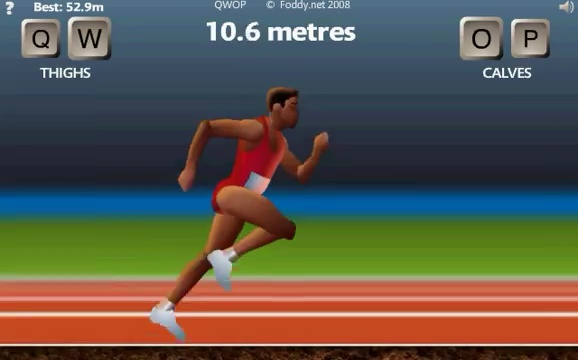
\includegraphics[scale=0.5]{240.jpg}}
\hspace{1cm}
\subfloat[DeepMind]{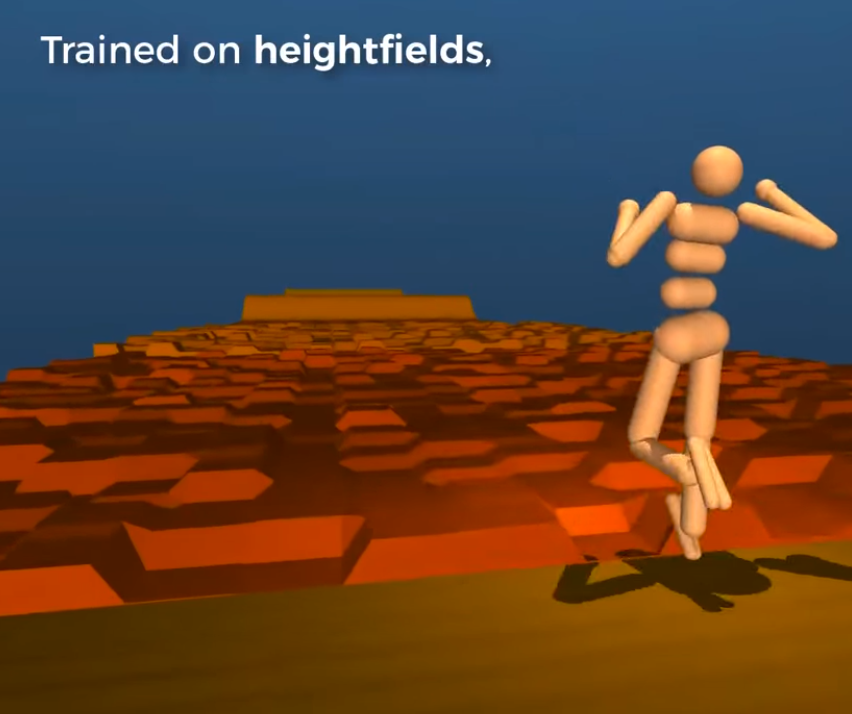
\includegraphics[scale=0.65]{deepmind.png}}
\hspace{1cm}
\subfloat[BipedalWalker]{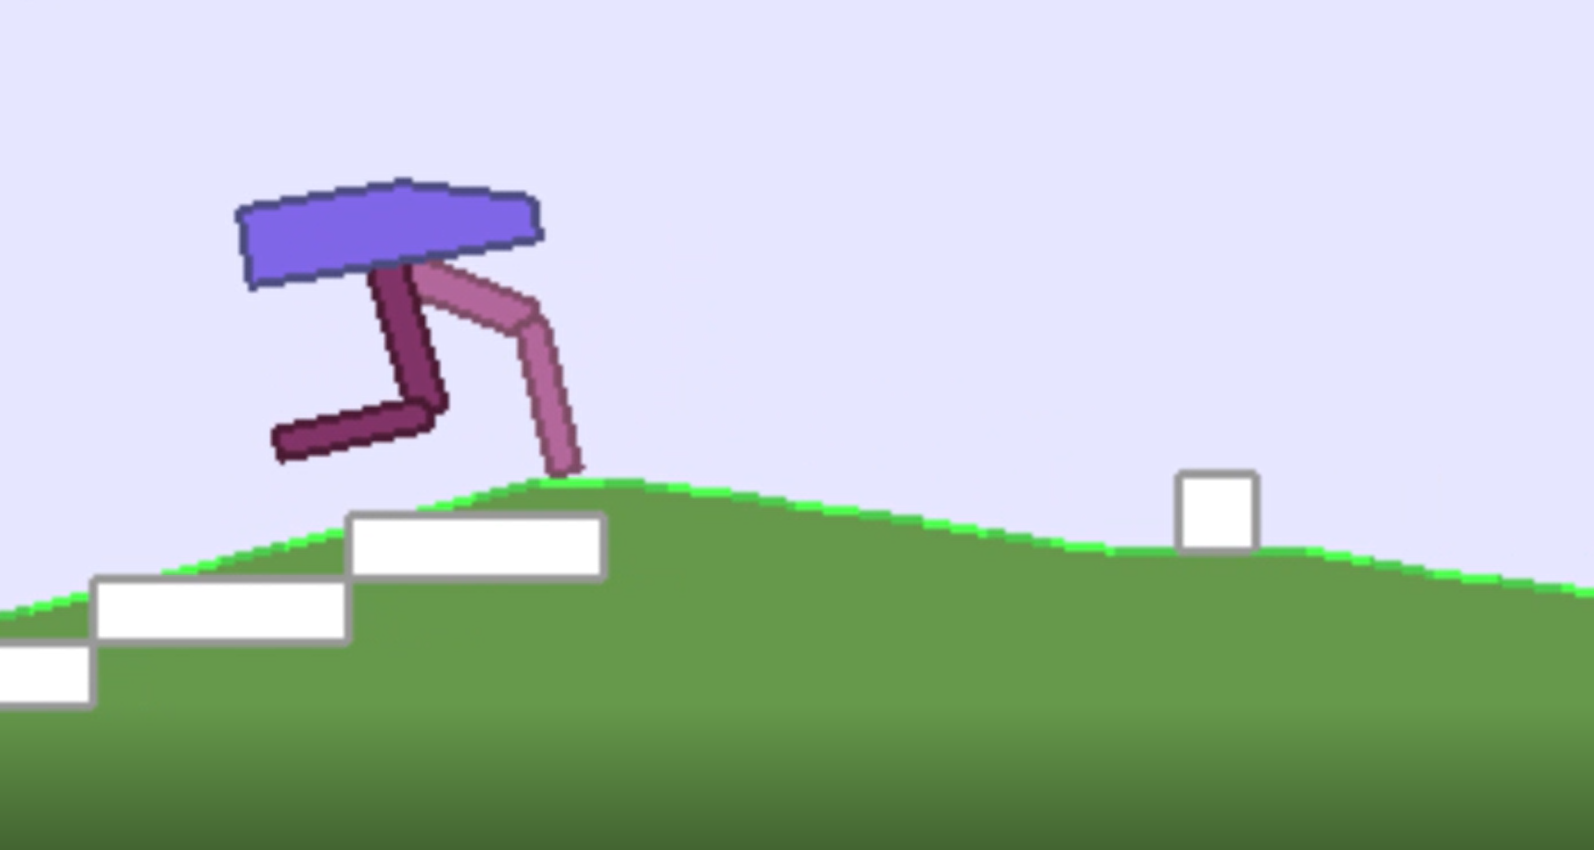
\includegraphics[scale=0.55]{bipedal_1.png}}
\end{figure}
}

\b

\block{Using DQN to play QWOP}{
%- Train a KNN classifier to recognize numbers and   use CNN to perform pose estimation from screenshot
% \begin{figure}[H]
% \ \ \ \ \ \ \ \ \ \
% 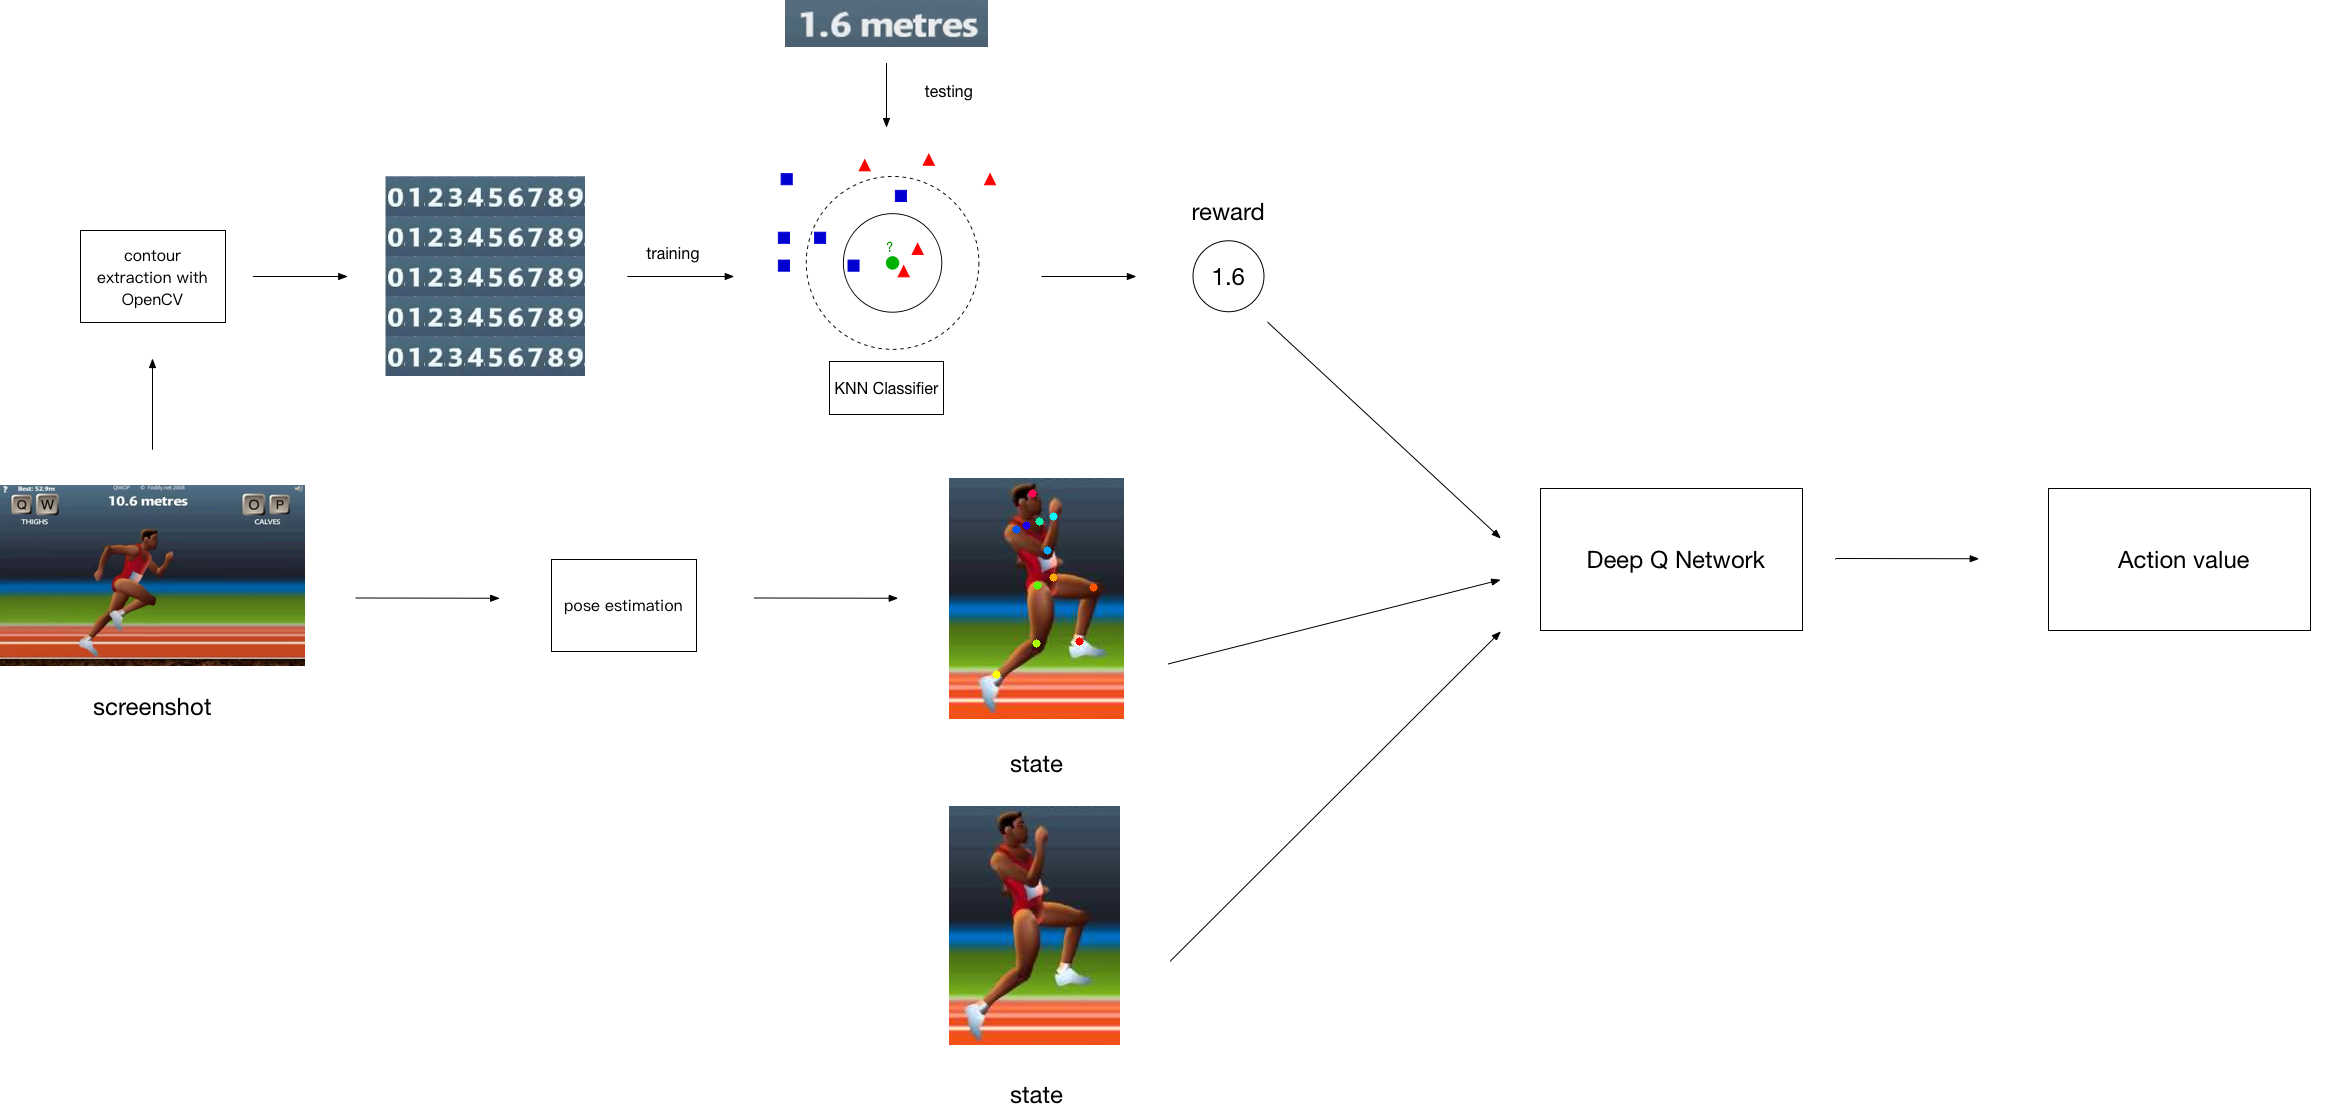
\includegraphics[scale=0.4]{DQN.png}
% \end{figure}
% - Use CNN + FC to Approximate the optimal action-value function
% \begin{equation*}
% %\tcboxmath{K_{k+1}=P_ka_{k+1}^T(a_{k+1}P_ka_{k+1}^T+I_N)^{-1}}

% \end{equation*}
% - Use Experience Play to Learn From the Past and Q-learning Update
% \begin{equation*}
% \tcboxmath{L_i(\theta_i) = \mathbb{E}_{(s,a,r,s') \scriptsize{\sim} U(D)}[(r + \gamma \max \limits_{a'}Q(s',a';\theta_i^-) - Q(s,a;\theta_i))^2]}
% \end{equation*}
% - Use uinput to simulate the process of press button since QWOP is a closed-sourced \\
% \begin{figure}[H]
% \ \ \ \ \ \ \ \ \ \ \ \ \
% 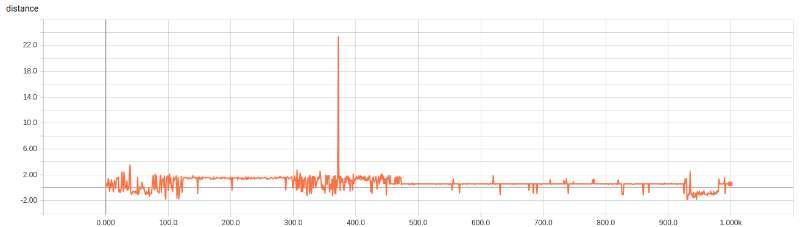
\includegraphics[scale=1]{DQN_distance2.jpeg}
% \end{figure}
% \centering
% \small{Fig: raw pixel as input of Deep Q Network}
\begin{figure}[H]
\ \ \ \ \ \ \ \ \ \ \ \ \ \ \ \ \ \ 
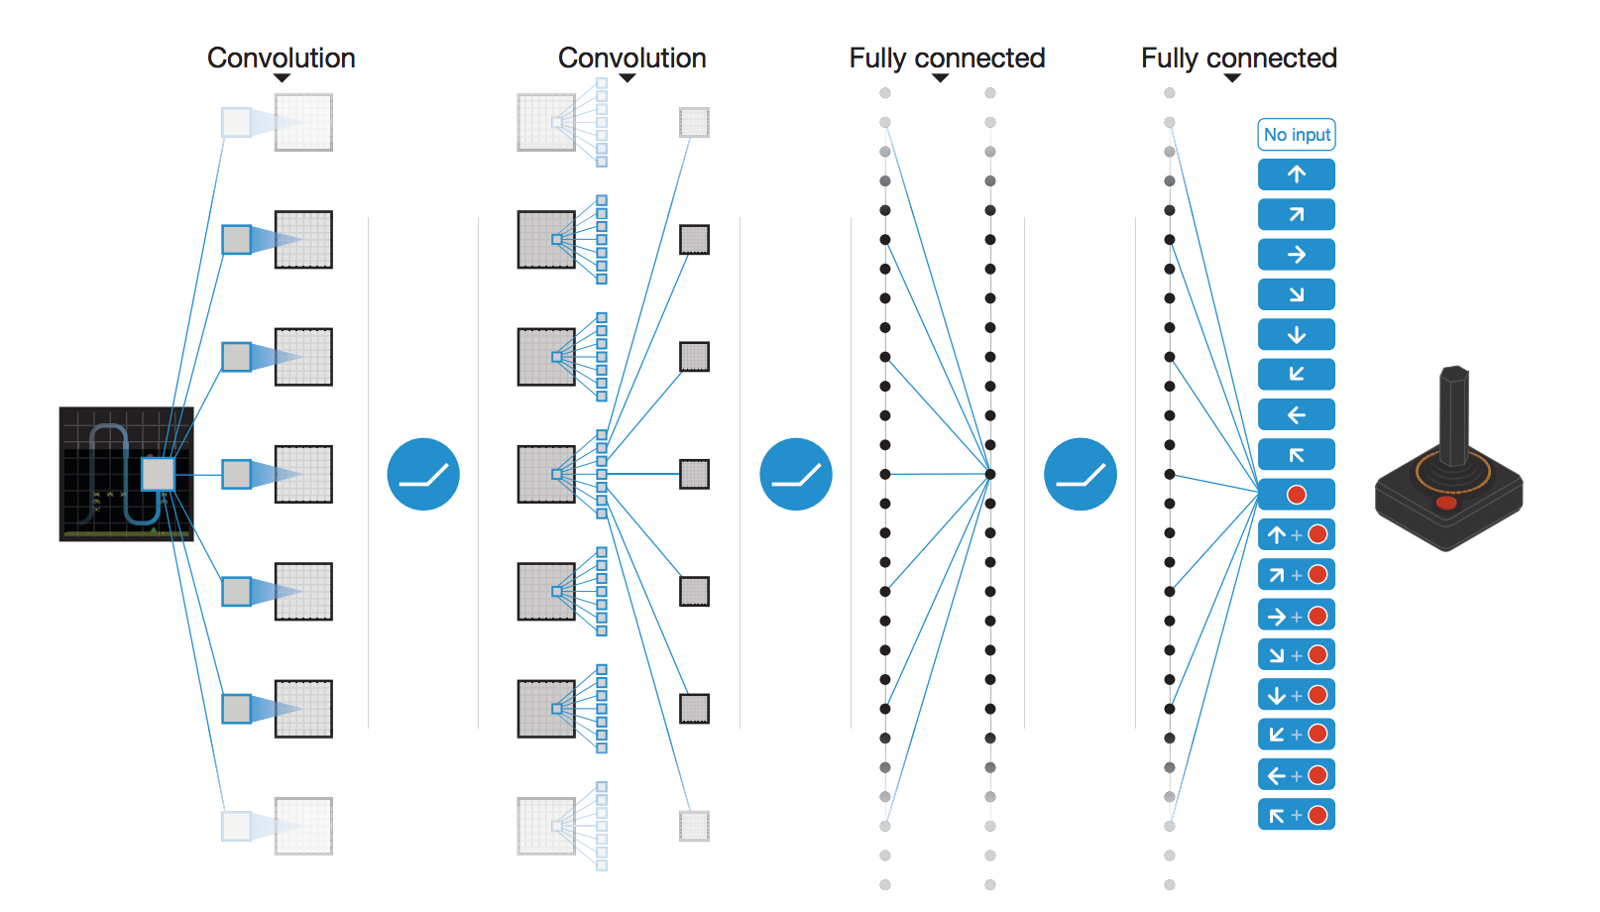
\includegraphics[scale=0.5]{dqn_net.png}
\end{figure}
- The goal of Q learning is to maximize long-term cumulative reward with Q value(action state value)
\begin{equation*}
\tcboxmath{$R_{t_0}=\sum_{t=t_0}^{\inf}\gamma^{t-t_0}r_t, Q^*(s,a) = \max \limits_{a} \mathbb{E}[r_t + \gamma r_{t+1} + \gamma^2 r_{t+2} + ...|s_t = s, a_t = a, \pi]}
\end{equation*}

- Use Experience Play to Learn From the Past and Q-learning Update
\begin{equation*}
\tcboxmath{L_i(\theta_i) = \mathbb{E}_{(s,a,r,s') \scriptsize{\sim} U(D)}[(r + \gamma \max \limits_{a'}Q(s',a';\theta_i^-) - Q(s,a;\theta_i))^2]}
\end{equation*}

}

\column{0.35}
\block{}{
% \begin{figure}[H]
% \ \ \ \ \ \ \ \ \ \
% 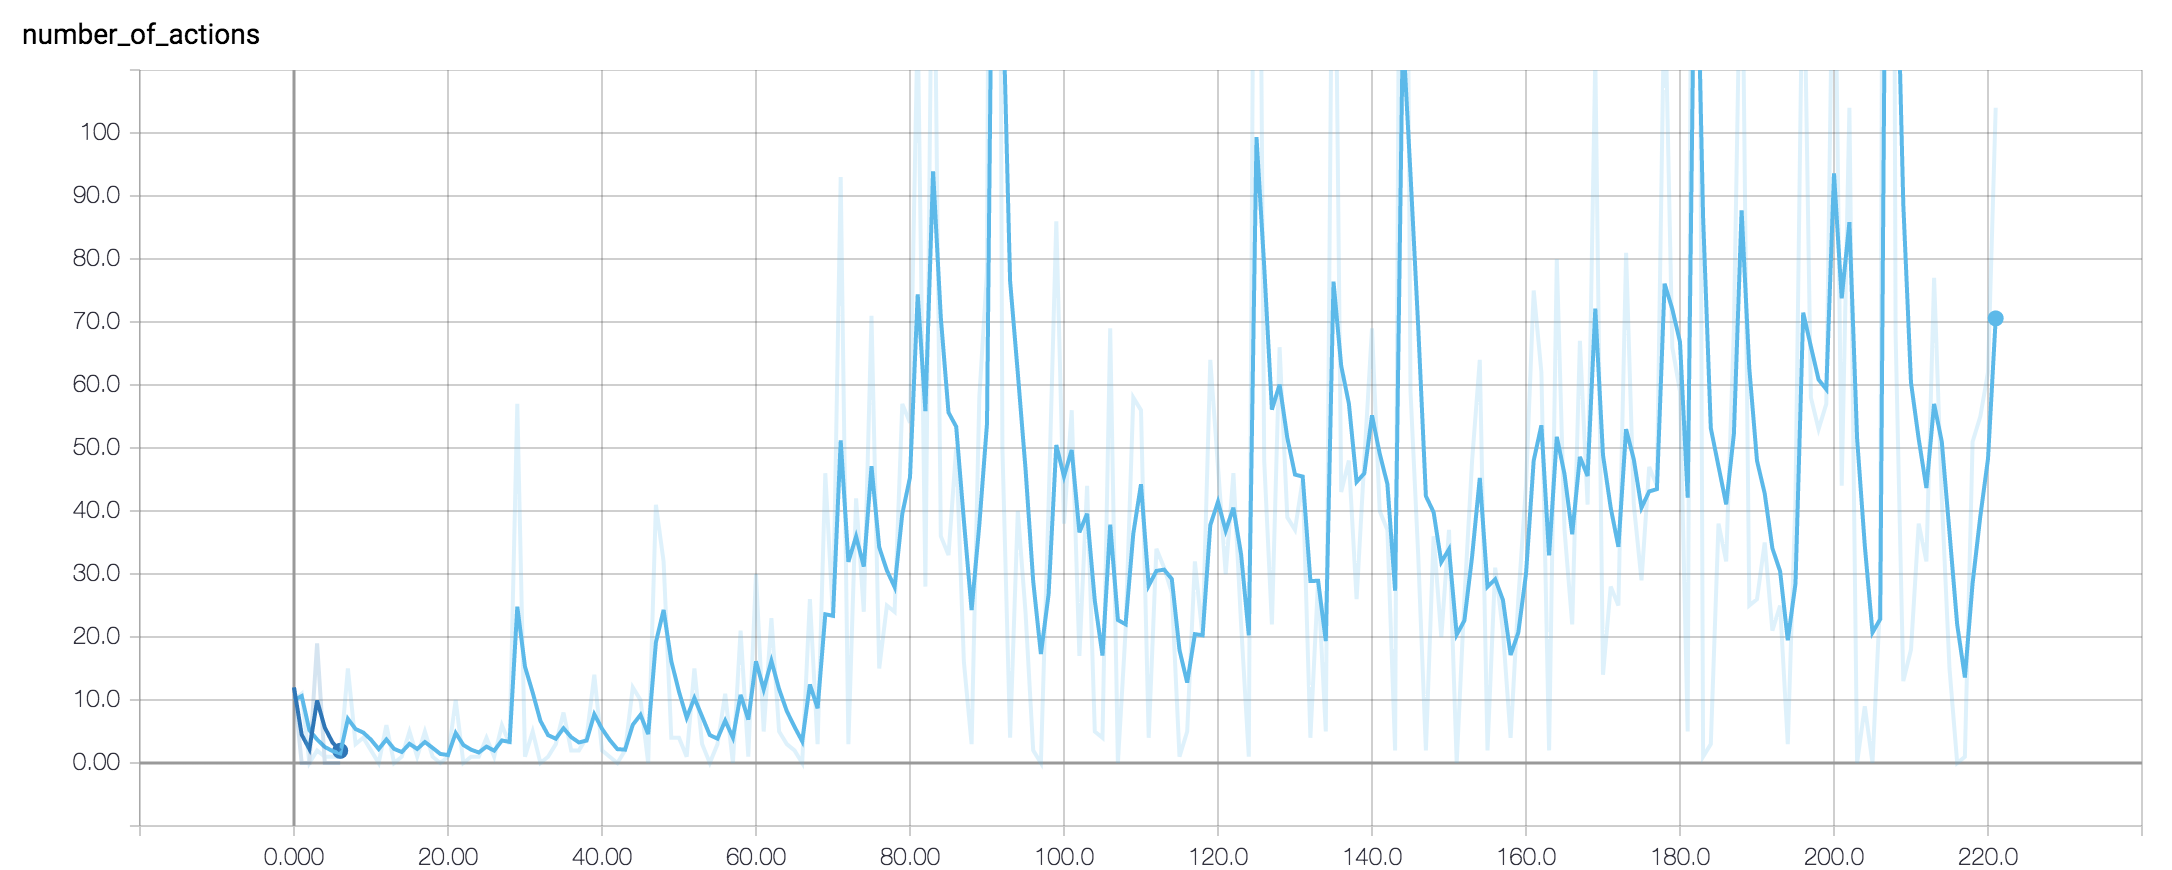
\includegraphics[scale=0.8]{DQN_distance3.png}
% \end{figure}
% \begin{center}
% \small{Fig: pose as input of Deep Q Network}
% \end{center}

\captionsetup[subfigure]{labelformat=empty}
\begin{figure}[H]
\ \ \ \ \ \ \ \ \ \ \ \ \ \ \ \ \
\subfloat[QWOP]{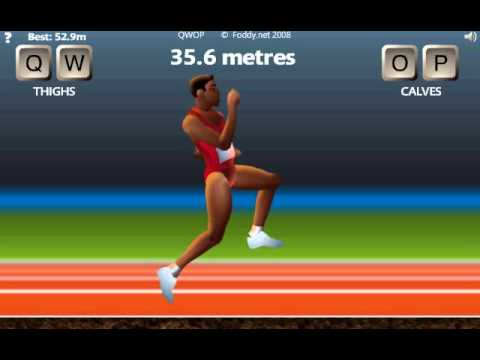
\includegraphics[scale=0.6]{qwop.jpg}}
\hspace{3in}
\subfloat[Pose Extraction]{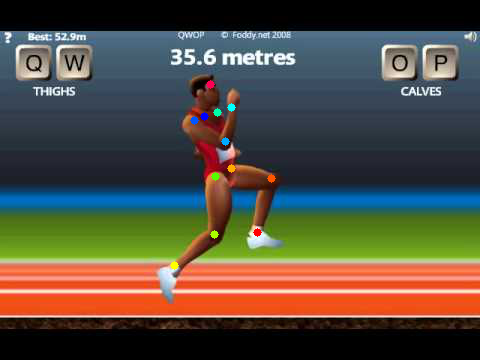
\includegraphics[scale=0.6]{result.png}}
\end{figure}
- Pretrained pose estimation model was used to predict moving joint from the screenshot of QWOP.

\begin{figure}[H]
\ \ \ \ \ \ \ \ \ \ \ \ \ \ \ \ 
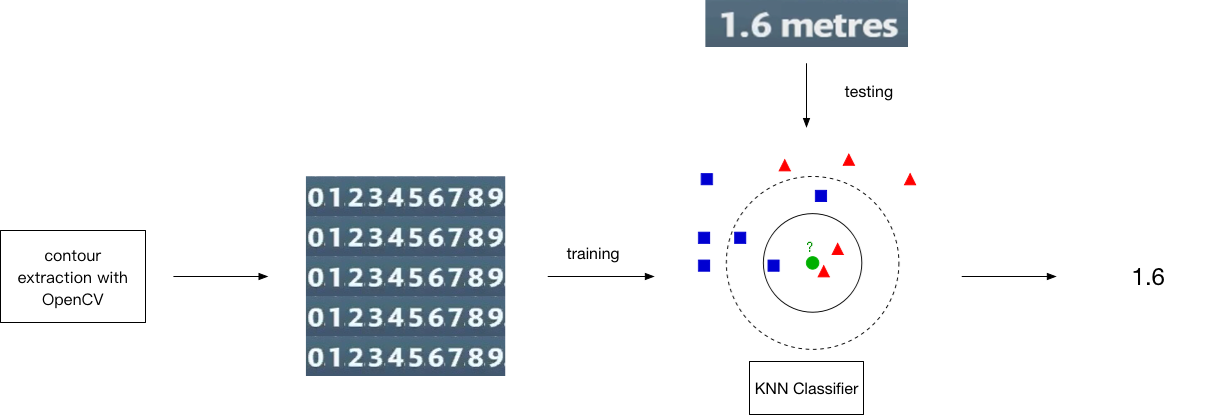
\includegraphics[scale=0.7]{OCR.png}

\end{figure}
- There is a time delay when pose estimation outputs flows into Q network, which greatly increase the trainging time.  \\
- Another problem is the training result is very unsastisfactory, possible reason for this could be there are only 16 combinations of inputs(considering to play QWOP
only four keys are needed), discrete action space may can not well represent the complex behaviour s likewalking. \\
- The last problem is QWOP is total blackboxed, whcih could indicatef that envrioment is not fully observable. 
}


\block{Problems when using DQN}{
\captionsetup[subfigure]{labelformat=empty}
\begin{figure}[H]
\ \ \ \ \ \ \ \ \ \ \ \ \ \ \ \ \ \ \ \ 
\subfloat[running distance wrt. episodes]{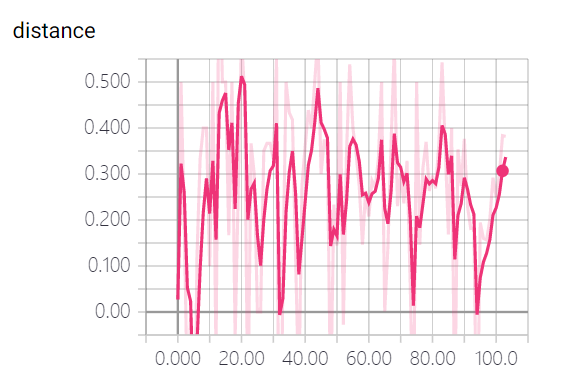
\includegraphics[scale=1.5]{dqn_xue.png}}
\hspace{3cm}
\subfloat[actions wrt. episodes]{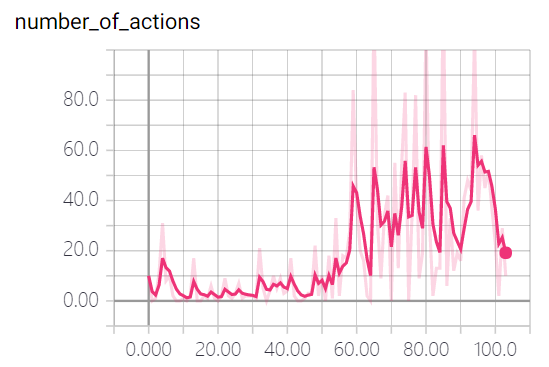
\includegraphics[scale=1.5]{dqn_xue1.png}}
\end{figure}
- QWOP is also too blackboxed, only partial observations could be correctly transfered to states. 

\begin{figure}[H]
\ \ \ \ \ \ \ \ \ \ \ \ \ \ \ \ \ \
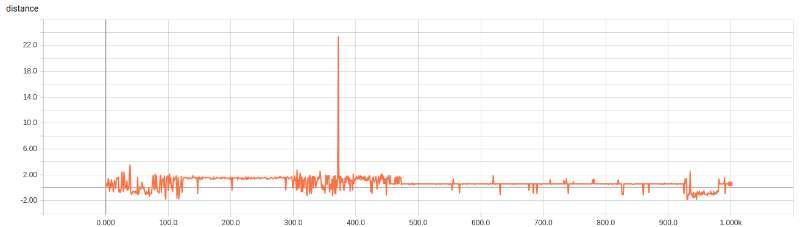
\includegraphics[scale=1]{DQN_distance2.jpeg}
\end{figure}

- Possible reason could be the discrete low-dimensional action space, since in QWOP there are only 16 combinations of inputs.

}


%\block{DDPG and PPO plays BipedalWalker}{
%At its core, DDPG is a policy gradient algorithm %that uses a stochastic behavior policy for good %exploration but estimates a deterministic target %policy, unlike DQN, it directlz learn a policy %function. 
%from the papar 
%\begin{figure}[H]
%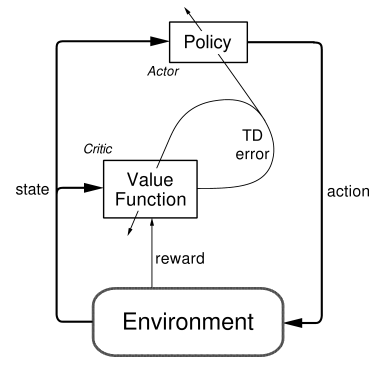
\includegraphics[scale = 0.8]{actor-critic.png}
%\end{figure}

    
    
% \textbf{DDPG} \\
% - Update critic by minimizing the loss
% \begin{equation*}
% \tcboxmath{L = \frac{1}{N} \sum_i(y_i - Q(s_i,a_i|\theta^Q))^2}
% \end{equation*}
% - Update actor policy using the sampled policy gradient
% \begin{equation*}
% \tcboxmath{\bigtriangledown_{\theta^{\mu}} J \approx \frac{1}{N} \sum \limits_i \bigtriangledown_a Q(s,a|\theta^Q)|_{s=s_i,a=\mu(s_i)} \bigtriangledown_{\theta^{\mu}} \mu(s|\theta^{\mu})|s_i}
% \end{equation*}
%}


\column{0.3}
\block{DDPG and PPO plays BipedalWalker}{
\textbf{DDPG} \\
\\
- DDPG introduce continuous action control into reinforcement learning, where actor part can be implemented with many different policy optimizations, PPO is one of the state of the art algorithm. \\

- Since QWOP is too bloackbox, we test our PPO implementation in Open AI gym's BipedalWalker environment. \\

\begin{figure}[H]
\ \ \ \ \
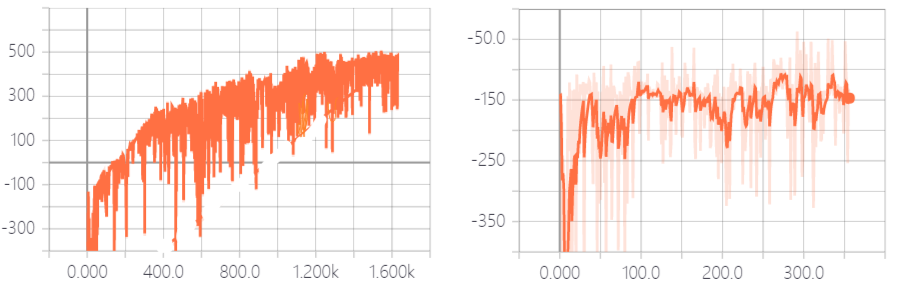
\includegraphics[scale=0.9]{PPO_comp.png}
\end{figure}

\textbf{PPO}\\
\\
- Agent could finish BipedalWalker-v environment within 1000 episodes. but even can't make any sound advances in hardcore environment, which includes 3 kinds of obstacles. \\
\captionsetup[subfigure]{labelformat=empty}
\begin{figure}[H]
\ \ \ 
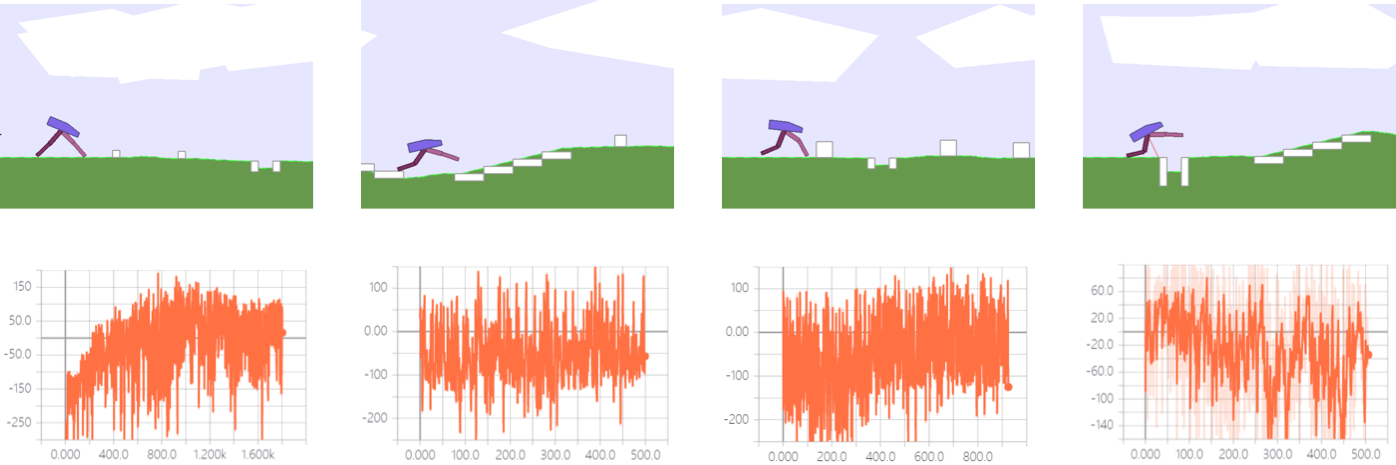
\includegraphics[scale=0.6]{PPO_reward.png}
\end{figure}
- We then tweaked the parameters of environment to procedurally generated tasks with increasing difficulties.\\
\\
- With increasing difficulties, agent's rewards remains in certain range, which could indicate that agent is able to overcome challenges with increasing abilities, just like human. \\


}





\block{Conclusion}{
- Modifying DQN with continuous output achieves better control result than discrete output \\
- The time cost of pose extraction has great influence on the performance \\
- Diversity of environment could help promoting the learning of agent
}








% \block{4. Reference}{
% \begin{thebibliography}{99}
% \bibitem{1}N. Heess, S. Sriram, J. Lemmon, J. Merel, G.Wayne, Y. Tassa, T. Erez, Z. Wang, A. Eslami, M. Riedmiller, et al. Emergence of locomotion behaviours in rich environments. arXiv preprint arXiv:1707.02286, 2017.
% \bibitem{2}T. Insider. Google’s deepmind ai just taught itself to walk. July 2017.
% \bibitem{3}T. P. Lillicrap, J. J. Hunt, A. Pritzel, N. Heess, T. Erez, Y. Tassa, D. Silver, and D. Wierstra. Continuous control with deep reinforcement learning. arXiv preprint arXiv:1509.02971, 2015.
% \bibitem{4}J. Merel, Y. Tassa, S. Srinivasan, J. Lemmon, Z. Wang, G. Wayne, and N. Heess. Learning human behaviors from motion capture by adversarial imitation. arXiv preprint arXiv:1707.02201, 2017.
% \bibitem{5}V. Mnih, K. Kavukcuoglu, D. Silver, A. Graves, I. Antonoglou, D. Wierstra, and M. Riedmiller. Playing atari with deep reinforcement learning. arXiv preprint arXiv:1312.5602, 2013.
% \bibitem{6}V. Mnih, K. Kavukcuoglu, D. Silver, A. A. Rusu, J. Veness, M. G. Bellemare, A. Graves, M. Riedmiller, A. K. Fidjeland, G. Ostrovski, et al. Human-level control through deep reinforcement learning. Nature, 518(7540):529–533, 2015.
% \bibitem{7}H. Su, C. R. Qi, Y. Li, and L. J. Guibas. Render for cnn.
% \bibitem{8}Z.Wang, J. S. Merel, S. E. Reed, N. de Freitas, G.Wayne, and N. Heess. Robust imitation of diverse behaviors. In Advances in Neural Information Processing Systems, pages 5324–5333, 2017.
% \end{thebibliography}
% }

\end{columns}
\end{document}
